%\begin{noindent}
\begin{markdown}
# Schaltanlagen

\GrayBox{Als **Schaltanlage** wird die Gesammtheit der Betriebsmittel (eines Ortes) bezeichnet, mit denen der **Strom** **verteilt**, **gemessen* oder **geschalten** wird - sowie die dazugehörigen **Schutz- und Steuereinrichtungen**. Ist ein **Transformator** vorhanden, spricht man von einer **Umspannanlage**.}

**Unterscheidung**

- Aufstellungsort
    - Innenraumschaltanlage
    - Freiluftschaltanlage
- Netzebene
    - Hochspannungsschaltanlage
    - Mittelspannungsschaltanlagen
    - Niederspannungsschaltanlagen
- Bauform
    - offene Bauform (Luftisolierung)
    - geschlossene Bauform

**Betriebsmittel einer luftisolierten Hochspannungsanlage:**

- Sammelschiene
- Schalteinrichtung
    - Trennschalter
    - Leistungsschalter
    - Lastschalter
    - Lasttrenner / Sicherung
- Wandler _(Strom- und Spannungswandler)_
- Sperrdrosseln und Kopplungskondensatoren 
- Überspannungsableiter

**Betriebsmittel einer gasisolierten Schaltanlage:**

- Sammelschiene
- Schalteinrichtung
- Wandler

## Schalteinrichtungen

\GrayBox{Schaltgeräte sollen dass öffnen von Stromkreisen _(in denen ein großer Strom fließt)_ ermöglichen, und den Lichbogen löschen.}

Es wird zwischen folgenden Schaltgeräten unterschieden:

- Trennschalter (oder Trenner)
- Leistungsschalter
- Lastschalter

**Ein Schaltgerät hat zwei Zustände:**

- offener Zustand _(dient als Isolierstrecke)_
- geschlossener Zustand _(muss den thermischen und mechanischen Beanspruchungen standhalten - inkl. Kurzschlussströme)_

**Mechanische Vorgänge beim Schalten**

- Das Schalten benötigt eine gewisse Zeit
- Durch trägheiten kommt es zum Schalterprellen
- Durch Verkleinerung der Masse und dadurch der Geschwindigkeit werden Lichtbögen begünstigt. _(Die mechanische Festigkeit wird geringer)_ 
- Schaltgeschwindigkeit bei Niederspannung ca. 10 cm/s, bei Hochspannung ca. 10 m/s

### Trennschalter

- Sehr Kleines Schaltvermögen
- **sichtbare Schalterstellung**
- Benötigt einen Schaltfehlerschutz _(um fehlerhaftes Schalten zu verhindern)_
- Wird nur ohne Betriebsstrom geschaltet _(würde beim auftretendem Lichtbogen zerstört werden)_
- Motorbetrieben
- Werden in **Freiluftschaltanlagen** verwendet
- Wird hin und wieder auch zum Erden von Anlagenteile verwendet

Beim betätigen des Trennschalters treten trotzdem schwache Lichtbogen auf, aufgrund der kapazitiven Blindströme.

### Lastschalter bzw. Lasttrennschalter

**Lastschalter**

- Sind nur für **Betriebsströme** ausgelegt _(Kurzschlussströme werden von Sicherungen oder Leistungsschalter übernommen)_

**Lasttrennschalter**

- **Lasttrennschalter** sind kombinierte Lastschalter und Trennschalter _(Lastschalter mit sichtbarer Trennstrecke)_
- Werden statt Trennschalter eingesetzt, zur **Erhöhung der Sicherheit**
- Werden in **kleinen Mittelspannungsverteilungsanlagen** eingesetzt
- Können auch in Netzen mit großen Strömen eingesetzt werden - benötigt aber Hochleistungssicherungen 

### Leistungsschalter

- Spezielle ein- oder dreipolige Schalter
- Sind für hohe Ströme ausgelegt _(bis 800kA)_ 
- Können auch **Kurzschluss und Ausschaltströme** ausschalten
- Kann mit folgenden Antrieben geschalten werden:
    - Magnetantrieb
    - Motorantrieb
    - Federantrieb
    - Druckluftantrieb

**Lichtbodenlöschungen:**

- Nullpunktlöschung
- Kurzschlusstromsbegrenzung

**Arten von Leistungsschalter**

- Öl-Arm _(Öl dient als Löschmedium vom Lichtbogen)_
- Druckluft _(Lichtbogen wird mit Luft weggeblasen)_
- SF6 _(Statt Luft wird mit Schwefelhexafluorid "gelöscht")_
- Vakuum
- Magnetblasschalter

\newpage

## Schaltlichtbogen

\GrayBox{Ein Lichtbogen entsteht beim **Öffnen** eines Schalters sowie beim **Durchschmelzen** von stromdurchflossenen Leitern oder beim **Durchschlag** einer Gasstrecke.}

Nur bei einer Spannung **unter 20V** kann **lichtbogenfrei** abgeschalten werden.

Durch den Lichtbogen wird er Schalter **thermisch hoch beansprucht** - besondere Maßnahmen sind erforderlich. 

Der Zusammenhang zwischen dem Druck und der Zündspannung für verschiedene Gase zeigt die **Paschenkurve**.

**Ablauf eines Lichtbogen:**

#. Hohe Temperaturen bilden ein Plasma
#. Durch Beschleunigung der Elektronen nimmt die Stromstärke zu
#. Das stromführende Plasma weist ab der Zündspannung einen fallenden (nicht linearen) Widerstand auf - Stromstärke wird größer.
#. Mit größer werdendem Abstand vergrößert sich die Lichtbogenlänge
#. Ist der Abstand zu groß, erlischt der Lichtbogen

### Gleichstromlichtbogen

Ein Gleichstromlichtbogen kann nur mit einem Vorwiderstand stabil brennen. Ohne Vorwiderstand wird die Spannungsquelle kurzgeschlossen.

\begin{wrapfigure}{r}{0.4\textwidth}
    \centering
    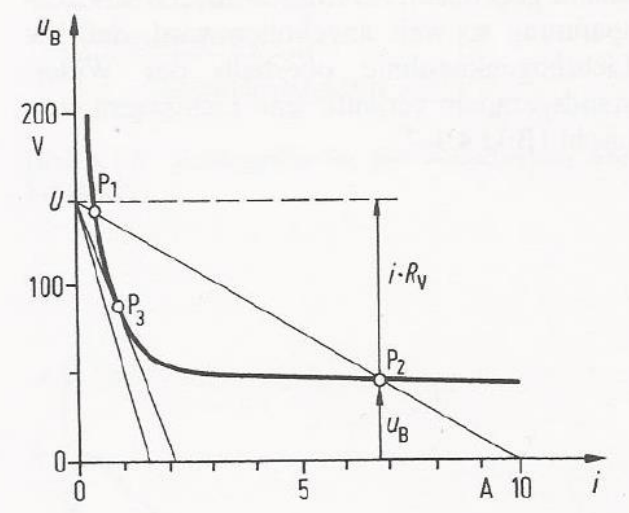
\includegraphics[width=\linewidth]{./images/10-Schaltanlagen/Lichtbogenkennlinie-Statisch.png}
    \caption[Statische Lichtbogenkennlinie]{Statische Lichtbogenkennlinie}
\end{wrapfigure}

**Je nach Größe des Vorwiderstandes lassen sich drei Fälle unterscheiden:**

Die Widerstandsgerade

- **schneidet die Lichtbogenkennlinie:** Es ergeben sich 2 Betriebspunkte - Der erste Punkt ist instabil, eine kleine Vergrößerung des Stroms führt allerdings dazu, dass der Strom bis Punkt 2 weiter ansteigt. Beim zweiten Punkt brennt der Lichtbogen stabil.  
- **tangiert die Lichtbogenkennlinie:** Instabiler Zustand - Der Lichtbogen kann bei jeder Änderung abreisen
- **verläuft unterhalb der Lichtbogenkennlinie:** Widerstand ist groß genug und die Spannung fällt daran ab

Wenn die Lichtbogenlänge vergrößert wird, rutscht die Kennlinie nach oben, sodass der Strom abnimmt.

**Maßnahmen zum Löschen:** _(Der Brennspannungsbedarf muss größer sein als die Treibende Spannung)_

- Lichtbogen verlängern
- Lichtbogen in mehrere Teilbogen unterteilen
- Säulenfeldstärke erhöhen _(Schalter kühlen)_
- Lichtbogensäule an Isolierstoffwände "drücken"
- Schnelle Kontakttrennung 

\newpage

### Wechselstromlichtbogen

Wechselstromlichtbogen folgen nicht der statischen Lichtbogenkennlinie. _(Es entstehen Verzerrungen der Lichtbogenspannung)_

Mit einem Wert eines sinusförmigen Stroms, kann die dazugehörige Lichtbogenspannung von der Hystereseschleife entnommen werden.

Der Verlauf der Lichtbogenspannung wird, abhängig von der Zeit, punktweise von der Hystereseschleife entnommen. 

Der gleiche Spannungsverlauf tritt in der nächsten Halbperiode mit umgekehrten Vorzeichen auf.

\begin{wrapfigure}{r}{0.5\textwidth}
    \centering
    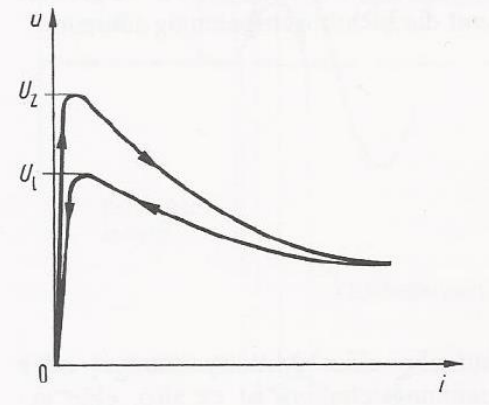
\includegraphics[width=0.8\linewidth]{./images/10-Schaltanlagen/Lichtbogenkennlinie-Dynamisch.png}
    \caption[Dynamische Lichtbogenkennlinie]{Dynamische Lichtbogenkennlinie}
\end{wrapfigure}

Nach jeder Halbperiode geht der Strom wieder auf null. Wenn man nach dem Nulldurchgang das Wiederentzünden des Lichtbogens verhindert, ist der Lichtbogen gelöscht. Nach diesem Prinzip arbeiten die **Nullpunktlöscher**

**Maßnahmen zum Löschen:** _(Die Wiederentzündungsspannung muss größer sein als die Netzspannung)_

- Intensiven Kontakt in Löschblechen
- Löschgasströmungen
- Vakuumschalter
- Schnelle Bewegung des Kontaktsystems _(so dass die Kontaktstücke beim Nulldurchgang einen Abstand haben, um die wiederkehrende Spannung zu halten)_

\vspace{3em}

## Lichtbogenlöscheinrichtungen

**Aufgaben von Lichtbogenlöscheinrichtungen:**

- Aufnahme der Lichtbogenenergie
- Verhindern des Überschlages zu benachbarten Anlagenteilen
- Erzeugen einer ausreichend hohen Lichtbogenspannung
- Entionisierung der Schaltstrecke nach Stromnulldurchgang

**Möglichkeiten zur Erhöhung der Lichtbogenspannung:**

- Druck auf den Lichtbogen
- Aufteilung des Lichtbogens
- Kühlung des Lichtbogens
- Verlängerung des Lichtbogens

### Verlängerung und Kühlung des Lichtbogens

\GrayBox{Ein horizontal brennender Lichtbogen wird nach oben gezogen. _(Durch die Wärmewirkung und der daraus folgenden Sogwirkung)_ Die Lichbogensäule wird verlängert und der Brennspannung erhöht sich.}

**Weitere Möglichkeiten zur Verlängerung des Lichtbogen:**

- Keile in der Schaltkammer _(aus Isolierstoff)_
- Magnetisches Feld _(abstoßende Wirkung)_

Bei einem Kurzschluss können die starken Magnetfelder das Schaltstück zusätzlich aufschleudern und somit die Ausschaltzeit verkürzen.

\newpage

### Aufteilung des Lichtbogens

\GrayBox{In der Nähe des Schaltstücks ist der Spannungsabfall in der Lichbogensäule um einiges größer.}

\begin{wrapfigure}[11]{r}{0.6\textwidth}
    \vspace{-1em}
    \centering
    \includegraphics[width=0.8\linewidth]{./images/10-Schaltanlagen/Lichtbogenlöschung.png}
    \caption[Lichtbogenlöschung durch Löschbleche]{Lichtbogenlöschung durch Löschbleche}
\end{wrapfigure}

Durch Teilung des Lichtbogens können daher viel größere Spannungsabfälle erzeugt werden. (Abhängig von der Teilstrecken-Anzahl)

Die Teilung erfolgt mit mehreren untereinander Isolierten Blechstücken. _(Der Lichtbogen wird durch die Sogwirkung in die Bleche gezogen)_

**Diese Methode wird bei Niederspannungsleistungsschaltern und Leitungsschutzschaltern angewendet.**

\vspace{3em}

### Druck auf den Lichtbogen und Kühlung des Lichtbogens

\GrayBox{Bei großen Strömen wird das Öl zersetzt und es entstehen Gasblasen, welchen den Lichtbogen kühlen und den Druck erhöhen.}

Durch die besondere Form der Schaltkammer, verläuft die Ölströmung quer durch die Lichtbogensäule, welche dadurch erlöscht wird.

Nach dem erlöschen des Lichtbogens wird der Druck wieder aufgebaut.

\end{markdown}

\begin{enumerate}
    \item[a] \textbf{Expansionskammer:} Querströmung wird durch Hilfskolben erzeugt
    \item[b] \textbf{Löschkammer:} Querströmung wird stromabhängig erzeugt 
    \item[c] \textbf{Löschkammer mit Schaltstift:} Querströmung wird durch die Bewegung des Stiftes erzeugt (beim ausschalten); Bei große Ströme entstehen Dampfblasen   
\end{enumerate}

\begin{figure}[H]
    \centering
    \includegraphics[width=0.8\linewidth]{./images/10-Schaltanlagen/Lichtbogenlöschen-Druck.png}
    \caption[Lichtbogenlöschung durch Druck und Kühlung]{Lichtbogenlöschung durch Druck und Kühlung}
\end{figure}

\newpage

%\begin{noindent}
\begin{markdown}

## Hochleistungssicherungen

### Niederspannungs-Hochleistungs-Sicherung (NH)

_bis 100kA Abschaltstrom; bis 630A Bemessungsstrom_

**Aufbau und Funktion:**

- 1 oder mehrere parallele Schmelzleiter
- Lotbrücke Schmilzt zeitverzögert
- Lichtbogen wird in mehrere zerlegt
- Umliegender Sand kühlt die Lichtbögen und löscht sie beim Nulldurchgang
- Darf nur vom Fachmann getauscht werden
- Sehr zuverlässig

### Hochspannungs-Hochleistungs-Sicherung (NH)

_Werden im Mittelspannungsbereich bis 36kV eingesetzt_

Werden in Kombination mit Last- oder Trennschaltern eingesetzt

**Funktion:**

- Bei einem Kurzschluss schmilzt der Schmelzleiter - Der Strom wird unterbrochen
- Ein Schlagstift wird ausgelöst
- Somit wird ein Lasttrenner aktiviert
- Und/Oder es wird eine Meldung gesendet

**Häufige Anwendungen:**

- In Transformatorkreisen
- In Motorstromkreisen
- In Kondensatorbänken
- Schutz von Spannungswandlern

## Niederspannungsschaltgeräte

**Zu den wichtigsten Niederspannungsschaltgeräten gehören:**

- Sicherungen _(Schraub- und NH-Sicherungen)_
- Leistungsschalter _(LS-, FI- und Leistungsschalter - Sind für hohe Schaltleistungen und geringer Schalthäufigkeit ausgelegt)_
- Schütze _(Fallen bei fehlender Steuerspannung wieder in die Ausgangslage zurück - Sind für niedrige Schaltleistungen und hoher Schalthäufigkeit ausgelegt)_

## Wandler

\GrayBox{Es gibt Spannungs- und Stromwadnler. Sie transformieren Spannung für Mess- und Schutzkreise und isolieren diese gegen Hochspannung.}

Es werden **induktive Wandler** und (über 110kV) **kapazitive Spannungsteiler** verwendet.

Kapazitive Spannungsteiler sind kostengünstiger.

**Ausführungen:**

- Mittelspannungsbereich: **Gießharzwandler**
- Hoch- und Höchstspannungsbereich: **Öl- und SF6-Wandler** 

\newpage

### Induktiver Spannungswandler (Gießharzwandler)

_Ausgangsspannung 100V, Nennleistung 5-300VA_

- Geringe Streuung
- Genaues Übersetzungsverhältnis
- Wird im Leerlauf betrieben
- Zerstörung bei Kurzschluss
- Einsatz für Innenraumanlagen _(bis 110kV)_

### Induktiver Spannungswandler (Ölwandler)

- Ölausdehnungssystem im Wandlerkopf
- Einsatz für Freiluftanlagen _(24 bis 245 kV)_

### Induktiver Spannungswandler (SF6-isoliert)

- Explosionssicher _(durch SF6-Gas)_
- Gleichbleibende Langzeitgenauigkeit
- Wartungsfrei
- Gasdichte (Isolationsfestigkeit) kann Fernüberwacht werden
- _(72,5 bis 800 kV)_

### Kapazitiver Spannungswandler

- Präzise Transformation auf messbare Größen
- Isolation zwischen Hoch- und Niederspannungsnetz _(mit Öl)_
- Können an die "Powerline Communication" angekoppelt werden
- Bei höheren Spannungen wirtschaftlicher als induktive Spannungswandler

\begin{figure}[H]
    \centering
    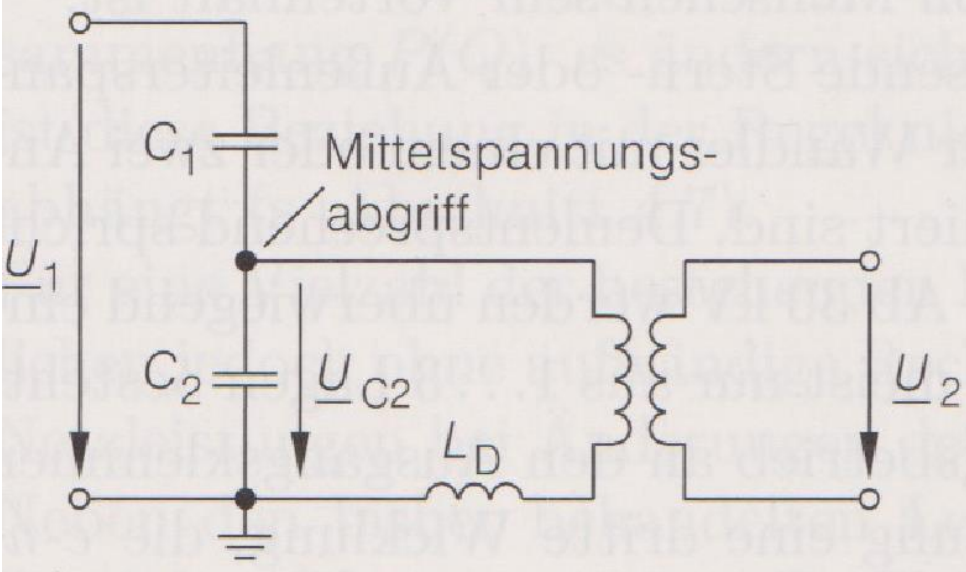
\includegraphics[width=0.4\linewidth]{./images/10-Schaltanlagen/Spannungswandler-Kapazitiv.png}
    \caption[Kapazitiver Spannungswandler]{Kapazitiver Spannungswandler}
\end{figure}

### Stromwandler

_Bemessungsstrom 1-5A, Bemessungsleistung 5-120VA_

- Werden primärseitig vom Hauptstrom durchflossen
- Nicht genau, aufgrund Nichtlinearität der Magnetisierungskennlinie
- Zerstörung bei Leerlauf _(Eisenkern überhitzt)_
- Betrieb im Kurzschluss oder niederohmiger Last

\begin{figure}[H]
    \centering
    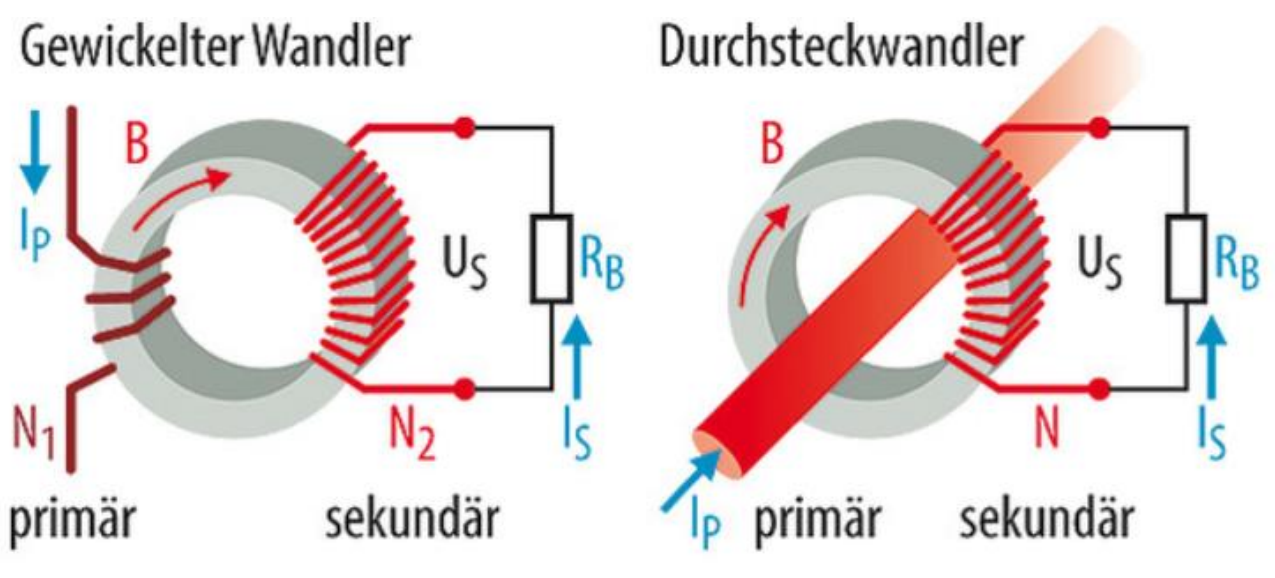
\includegraphics[width=0.6\linewidth]{./images/10-Schaltanlagen/Stromwandler.png}
    \caption[Stromwandler]{Stromwandler}
\end{figure}

\newpage

### Kombinierter Strom/Spannungswandler (SF6-isoliert)

- Explosionssicher _(durch SF6-Gas)_
- Kann bei hohen Kurzschlussströmen betrieben werden
- Gleichmäßig verteilte Sekundärwicklung
- Gleichbleibende Langzeitgenauigkeit
- Wartungsfrei
- Gasdichte (Isolationsfestigkeit) kann Fernüberwacht werden
- _(bis 800 kV)_

## Strombegrenzer / Drosselspulen

\GrayBox{Wenn ein Stromnetz nachträglich erweitert wird, Steigt auch die Kurzschlussleistung. Um vorhandene Leistungsschalter weiterhin zu verwenden, werden Kurzschlussstrombegrenzer _(z.B.: Drosselspulen)_ eingesetzt.}

Verbinden meistens Sammelschienenabschnitte (auf der Mittel- und Hochspannungsebene)

**Aufgaben:**

- Reihendrosselspule: Begrenzung von Kurzschlussströmen
- Ladestromdrossel: Kompensation von kapazitiven Ladestrom in Leitungen
- Einphasige Drosselspulen: Zur Erdung von Transformator-Sternpunkten
- In Stromrichteranlagen: Zur Glättung des Gleichstromes / Kurzschlussstrom Begrenzung

%? ## Kondensatoren

## Sperrdrosseln und Kopplungskondensatoren

\GrayBox{Hochspannungsleitungen werden auch oft zur Nachrichtenübertragung (mittels TFG) verwendet. Mit **Sperrdrosseln** werden Hochfrequente Signale blockiert.}

TFH Signale können jedoch Funkdienste stören. Deshalb wurde die Nachrichtenübertragung auf Richtfunksysteme oder Glasfaserkabel _(im Erdseil)_ umgestellt.

## Überspannungsableiter

Zum schutz vor Überspannungen durch Blitzeinschläge, werden Überspannungsableiter eingesetzt.

\GrayBox{Überspannungsableiter sind Bei Nennspannung isolierend, werden bei Überspannung jedoch leitend.}

**Entstehung von Überspannungen:**

- Direkte oder indirekte Blitzeinschläge
- Schaltvorgänge an Transformatoren, Motoren, Schützschaltern

## Sammelschiene

\GrayBox{Als Sammelschienen werden **Seile** oder **Rohrausführungen** verwendet _(für leistungsstarke Anlagen)_}

Es wird zwischen **Einfach- und Doppelsammelschienenanlage** unterschieden.

Die Anlage wird in Felder aufgeteilt:

- Einspeisefeld
- Abgangsfeld
- Kuppelfeld
- Messfeld

### Einfachsammelschiene

Vorteile: **Übersichtlich, Kompakt, Billig**

**Grundlegender Aufbau:** Reihenschaltung von Sammelschienentrenner, Leistungsschalter, Stromwandler, Spannungswandler und Erdungstrenner _(dient bei abgeschalteter Leitung zur Entladung von Freileitungskapazitäten)_.

\begin{figure}[H]
    \centering
    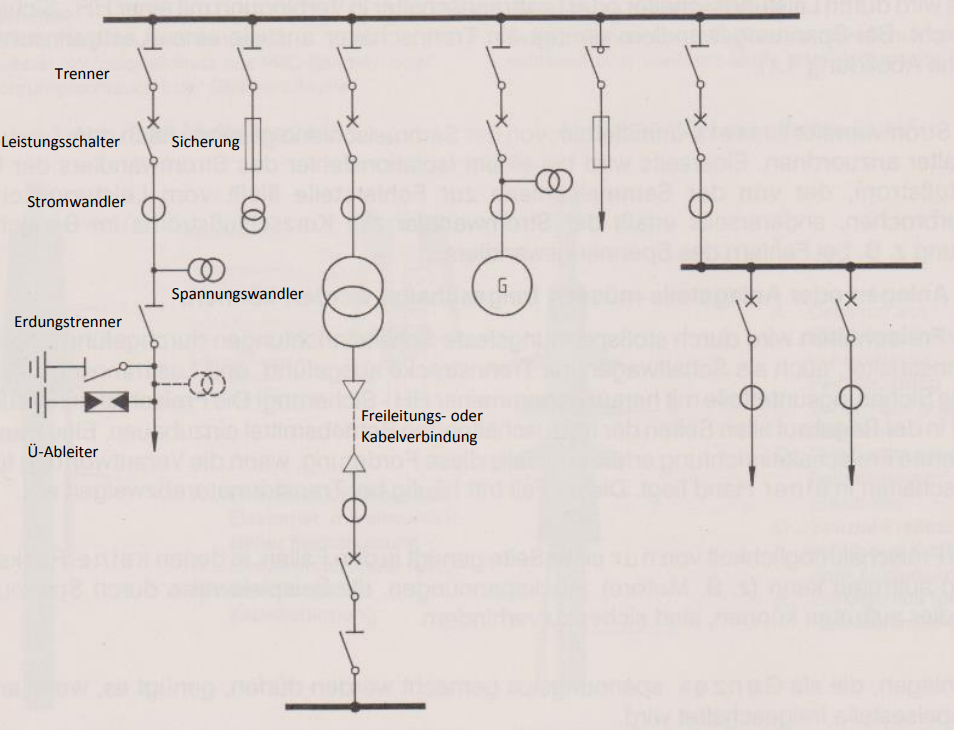
\includegraphics[width=0.9\linewidth]{./images/10-Schaltanlagen/Einfachsammelschiene-Aufbau.png}
    \caption[Einfachsammelschiene]{Einfachsammelschiene}
\end{figure}

**Einfachsammelschiene mit und ohne Längstrennung**

\end{markdown}

\begin{figure}[H]
    \centering
    \begin{subfigure}[t]{0.4\textwidth}
        \centering
        \raisebox{6mm}{
            \includegraphics[width=\textwidth]{./images/10-Schaltanlagen/Einfachsammelschiene-mit-Längstrennung.png}
        }
        \captionsetup{singlelinecheck=off}
        \caption[Ohne Längstrennung]{\textbf{Ohne Längstrennung}
            \begin{itemize}
                \item bei kleinen Anlagen üblich
                \item kompletter Ausfall bei Wartungen
            \end{itemize}
        }
    \end{subfigure}
    \hspace{1cm}
    \begin{subfigure}[t]{0.4\textwidth}
        \centering
        \includegraphics[width=\textwidth]{./images/10-Schaltanlagen/Einfachsammelschiene-ohne-Längstrennung.png}
        \captionsetup{singlelinecheck=off}
        \caption[Mit Längstrennung]{\textbf{Mit Längstrennung}
            \begin{itemize}
                \item Teilbetrieb bei Wartungen möglich
            \end{itemize}
        }
    \end{subfigure}
    \caption[Einfachsammelschiene mit und ohne Längstrennung]{Einfachsammelschiene mit und ohne Längstrennung}
\end{figure}

\newpage

%\begin{noindent}
\begin{markdown}

### Doppelsammelschiene (mit Kupplung)

- Teilbetrieb bei Wartungen möglich
- Last kann auf zwei Teilnetze aufgeteilt werden
- Asynchroner Betrieb möglich
- Mit Kuppelschalter können Lasten auf eine andere Schiene umgeschalten werden 

\begin{figure}[H]
    \centering
    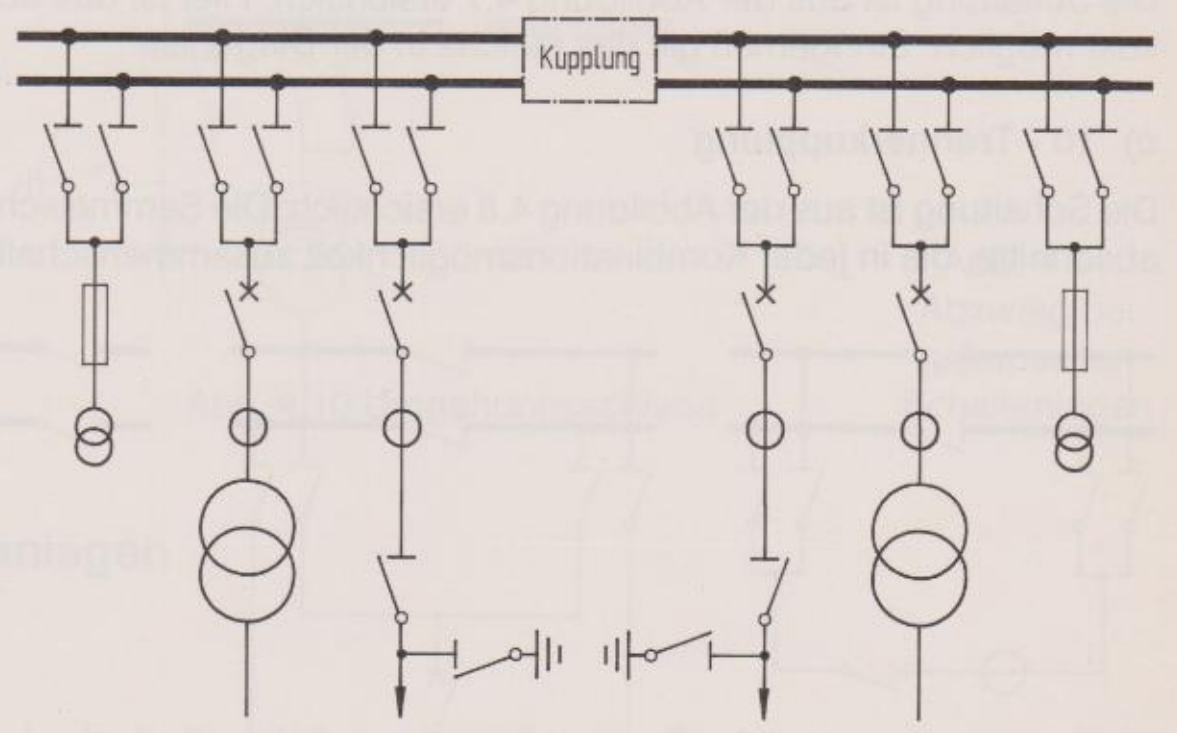
\includegraphics[width=0.6\linewidth]{./images/10-Schaltanlagen/Doppelsammelschiene.png}
    \caption[Doppelsammelschiene]{Doppelsammelschiene}
\end{figure}

### Kupplungen von Sammelschienen

\end{markdown}

\GrayBox{Durch Leistungsschalter werden zwei Sammelschienen verbunden. - Es können unabhängige Netze miteinander verbunden werden.}

\noindent
\begin{minipage}[t]{0.3\textwidth}
    \textbf{Querkupplung}

    \begin{figure}[H]
        \centering
        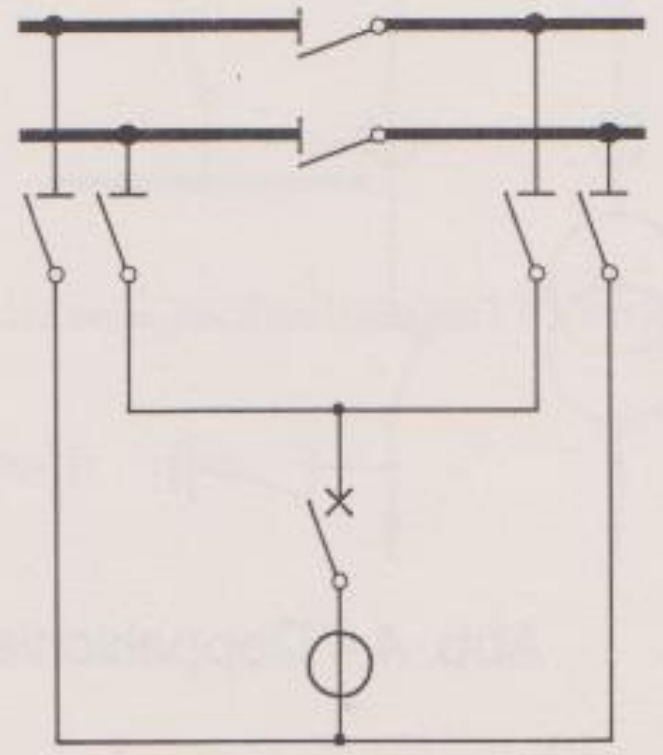
\includegraphics[width=0.7\textwidth]{./images/10-Schaltanlagen/Querkupplung.png}
        \captionsetup{singlelinecheck=off}
        \caption[Querkupplung]{\newline Querkupplung}
    \end{figure}

    Schalten in Querrichtung und Längsrichtung möglich. (nicht diagonal)
\end{minipage}%
\hspace{0.05\textwidth}%
\begin{minipage}[t]{0.65\textwidth}
    \noindent
    \begin{minipage}[t]{0.45\textwidth}
        \textbf{Längskupplung}

        \begin{figure}[H]
            \centering
            \includegraphics[width=0.7\textwidth]{./images/10-Schaltanlagen/Längskupplung.png}
            \captionsetup{singlelinecheck=off}
            \caption[Längskupplung]{\newline Längskupplung}
        \end{figure}
    
        Schalten in Längsrichtung und Diagonal möglich.
    \end{minipage}%
    \hspace{0.1\textwidth}%
    \begin{minipage}[t]{0.55\textwidth}
        \textbf{Einfache Querkupplung}

        \begin{figure}[H]
            \centering
            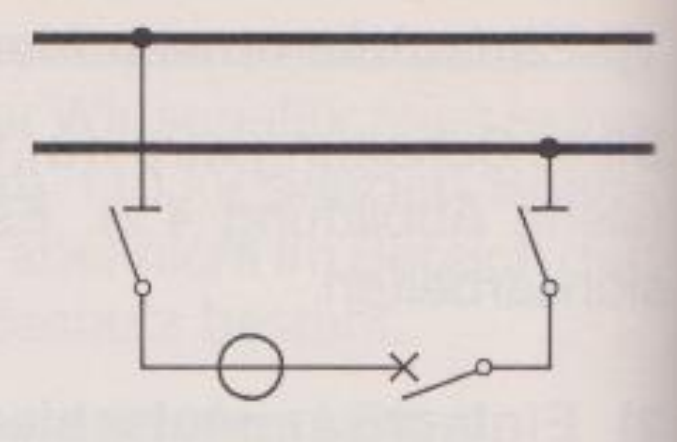
\includegraphics[width=0.7\textwidth]{./images/10-Schaltanlagen/Querkupplung-Einfach.png}
            \captionsetup{singlelinecheck=off}
            \caption[Einfache Querkupplung]{\newline Einfache Querkupplung}
        \end{figure}
    \end{minipage}

    \vspace{1em}

    \textbf{Umgehungsschiene mit einfacher Querkupplung}

    \begin{figure}[H]
        \centering
        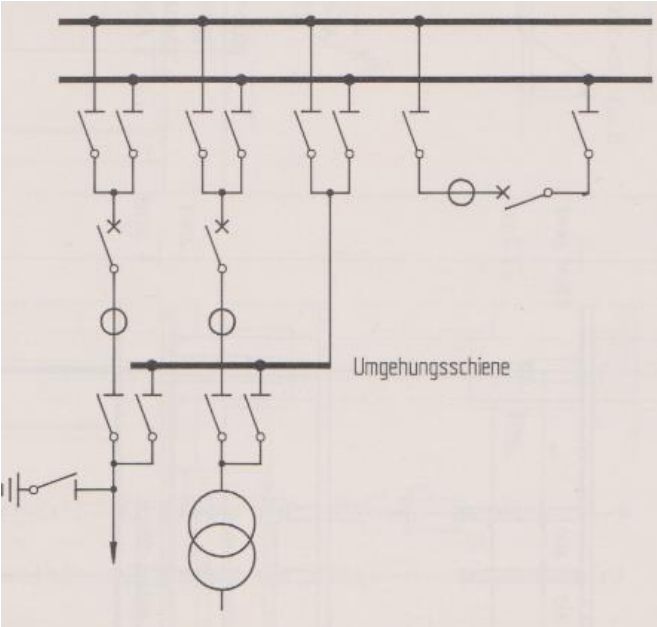
\includegraphics[width=0.6\linewidth]{./images/10-Schaltanlagen/Umgehungsschiene-mit-Querkupplung.png}
        \caption[Umgehungsschiene mit einfacher Querkupplung]{Umgehungsschiene mit einfacher Querkupplung}
    \end{figure}
\end{minipage}

\newpage

\begin{markdown}

## Spannungsschaltanlagen - Grundregeln nach ÖVE

#. **Einfache und Übersichtliche** Schaltung _(Sammelschienen)_
#. **Schalten von Betriebs- und Kurzschlussströmen** muss durchführbar sein. _(Leistungstrennschalter)_
#. Anlagenteile müssen **freigeschalten** werden können. _(Trennschalter oder Lastrennschalter)_
#. Jeder trennbare Abschnitt (Netz) muss eine **Spannungsmesseinrichtung und Erdschlussanzeige** besitzen
#. Jeder Anlagenteile muss **geerdet und kurzgeschlossen** werden können

## Hochspannungsschaltanlagen

_Ölarme- und Druckluft-Schalter sowie Öl-isolierte Wandler wurden auf die SF6-Technologie umgestellt_ 

**Aufbau**

- Kapazitiver Teiler _(zum ein-/aus-koppeln der Trägerfrequenz - um Nachrichten zu senden)_
- Abzweigfeld
    #. Leitungstrennschalter
    #. Strom- und Spannungswandler
    #. Leistungsschalter
    #. Sammelschienentrennschalter
- Sammelschienen
- Überspannungsableiter

Bei leistungsstarken Anlagen wird für die Sammelschiene eine Rohrausführung verwendet, ansonsten Leiterseile.

## Hochspannungsschaltanlagen (SF6-Ausführung)

\GrayBox{Alle Anlagenteile _(Sammelschiene, Trenner, Schalter, Wandler und Kabelverschlüsse)_ sind in geerdeten Kapselungen untergebracht und mit SF6-Gas gefüllt.}

_Deckt den gesamten Spannungsbereich von 6 bis 800 kV ab._

- Unbrennbar, Explosionssicher _(durch SF6-Gas)_
- Kompakt gegenüber Freiluftanlagen
- SF6-Gas dient auch zur Lichtbogen-Löschung
- Durch **Lichtbögen und Teilladungen entstehen giftige Stoffe** - Muss bei Servicemaßnahmen beachtet werden

## Mittelspannungsschaltanlagen

**Typische Ausführungen:**

- Luft-isoliert und metall-gekapselt
- SF6-isoliert und gekapselt

Es werden SF6-Schalter oder Vakuumschalter eingesetzt.

\end{markdown}